\section{A felület elérése}

A kliens oldali program két féle módon is elérhető a felhasználók számára:
\begin{itemize}
  \item Tetszőleges internetböngészővel rendelkező eszközről a helyi hálózaton
  futó szerver segítségével. Ekkor a böngésző címsorába beírva a szerver címét
  egyből a FlockWave kliens felületét kapjuk, ami egy SPA (Single Page
  Application), tehát összesen egy lapból áll, nem alkalmaz navigációt.
  \item Windows, Linux vagy MacOS (OSX) rendszerek alatt Electron segítségével
  becsomagolt állománnyal rendelkező önálló alkalmazásként.
\end{itemize}

A felület megnyitása után szükséges csatlakozni a drónokkal történő közvetlen
kommunikációt végző FlockWave szerver alkalmazást futtató számítógéphez. Ez
lehetséges az elérési cím és port (alapértelmezetten 5000) manuális megadásával,
illetve az SSDP (Simple Service Discovery Protocol) hálózati felderítési
protokoll segítségével.

\section{A felület kezelése}

Alapállapotban a felület a térképet jeleníti meg, mellette pedig a rétegek
kezelésére alkalmas panelt, valamint az ismert drónok listáját. További felületi
elemek érhetőek el a fülekre kattintva, illetve a bal oldalon található sávról
kattintással vagy húzással a felületre helyezve.

\begin{figure}[h!]
  \center
  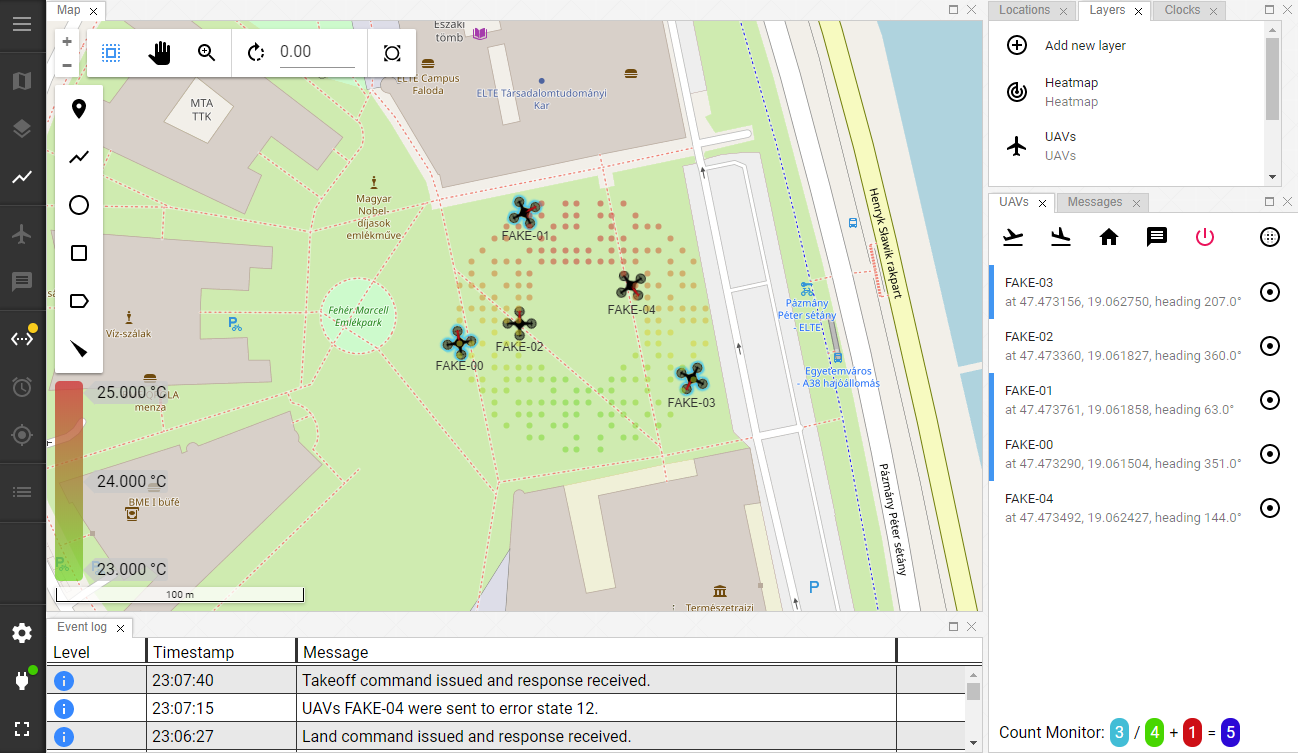
\includegraphics[width=\textwidth]{default_client_state.png}
  \caption{A kliens program alapállapota}
  \label{fig:default_client_state}
\end{figure}

// TODO: Panelek egyenként bemutatva és illusztrálva.
